\documentclass{article}
\usepackage[utf8]{inputenc}

\usepackage[margin=2cm]{geometry} % adjust margin
\usepackage{paralist} %compact itemize / enumeration
\usepackage{hyperref} %\url
\usepackage{numprint} %print numbers with thousand separator

\usepackage{graphicx}
\usepackage{wrapfig}
\graphicspath{ {./images/} }

\title{UfoVis}
\author{Marius, Philip, Robin}
\date{February 2021}

\begin{document}

\maketitle

\begin{itemize}
    \item Paper Outline Guidance (5-7 pages with graphics).
    \item Introduction.  Briefly describe the problem you are solving and a high-level description of your approach.  Include your motivation for this problem.  Why is it important and why should I care? 
    \item Data set.  Describe you data set in detail, how you collected the data and any preprocessing, data cleaning, transformations, etc.
    \item Methodology
    \begin{itemize}
        \item How did you use the data?
        \item What algorithms did you use and why?
        \item How does your approach help you solve problems you identified in the introduction?
    \end{itemize}
    \item System.  Describe the essential components of your system/application.  Include a description of the users of your system and the tasks they can perform or the questions they can answer.
    \item Use Cases.  Present one or two use cases that show case the most important features of your system.
\end{itemize}


\section*{Datasets}
There are two datasets that can be used in the project to display airports, depending on the amount of airports that should be included in the database.
\begin{compactenum}[1.]
\item The first dataset is from \url{https://www.abflug.info/} and contains approximately \numprint{6500} airports. All the airports have an IATA code and an ICAO code, other airports are not included in the dataset. The dataset additionally contains an identifier, the name in english and german, the length of the largest runway in feet, a link to the wikipedia entry in german and english, and the latitude, the longitude, the elevation in feet, and the \textit{ISO 3166-1 alpha-2} (country) code.\\
Because only larger airports have an IATA code and an ICAO code, there will be no differentiation between different airport types in the visualization when using this dataset, which means you can only see whether there is an airport near an UFO sighting.
\item The second dataset is from \url{https://ourairports.com/} and contains approximately \numprint{62000} airports. The dataset additionally contains an id, the type, the latitude, longitude and elevation, the name, the continent code, the \textit{ISO 3166-1 alpha-2} code, the \textit{ISO 3166-2} (region) code, the municipality, the name of the airport, whether there is scheduled service, the gps code, the IATA code, a local code, a link to the official website of the airport, a wikipedia link to the airport, and some keywords.\\
Because of the type attribute, this dataset has a differentiation between different airport types like small airports, large airports, or balloon ports.
\end{compactenum}
Both datasets were downloaded as \textit{.csv} file and transformed to sql insert statements. There was no data preprocessing done for them, except for replacing undefined values with null, and replacing the apostrophes such that the database can handle the values. Both datasets will also not be fully loaded into the database. Only the following important attributes are loaded into the database. The id, the name of the airport in english, the country code, the type, the coordinates and the elevation in feet.\\

The UFO reports were scraped from the website of the National UFO Reporting Center (NUFORC). Its an american organization, that collects and investigates alleged UFO sighings. On the NUFORC website (\url{http://www.nuforc.org/}), there is a link to a "report database" which is a collection of very basic HTML tables. You can choose different methods of indexing the database and then you get to a big list of links, all containing data. To automate this, we first collected all the urls to the data in HTML table form. Then we created node.js scripts to first download, then process and later upload the data to our own database. This process was very laborious because the HTML table was differently formatted in some cases and often unclosed tags. This confused some parsing libraries because they expect well formatted HTML. After this was fixed using some regex we had a big csv file with about 90 thousand reports. However, there was another problem. The reports only specify the location using the name of the city and without coordinates and it's also not known which country this reported city is in. To display markers on a map we needed to get the coordinates. To solve this we used a dataset of the biggest cities in the world and we were able to map the data to coordinates, sadly loosing about 20 percent of reports in the process, where no city could be found. The data was then transformed into sql insert statements and uploaded using a database connection. This process is fully automated and takes only a few seconds. 



%https://blog.mapbox.com/clustering-millions-of-points-on-a-map-with-supercluster-272046ec5c97
%https://github.com/Leaflet/Leaflet.markercluster
%https://d3js.org
\section*{Methodology}
Both datasets, the UFO report dataset and the airport dataset, were visualized on a map, to recognize patterns in the data. There were two attempts.\\
The first attempt was the creation of a heatmap based on the UFO data. The heatmap thereby highlighted places, where lots of UFOs were reported, but didn't lead to a recognition of patterns. Therefore a cluster map with glyphs was created.\\
This was the second attempt to discover patterns. For this visualization, parts of the UFO data and the whole airport data are loaded from the database. Each entry thereby has a marker on the geographic position of the event.
Because a lot of markers would most likely crash the system, you are not able to see whether there are makers on the same exact position, and it is hard to find patterns, a clustering algorithm was chosen to cluster events in close distance. The clustering is done by the leaflet library ''markercluster''. It uses a hierarchical greedy clustering approach. This approach selects a random marker from all the markers on the map and clusters all points within a specified distance (here: default, 80 pixel) to this marker. Further, it iteratively selects markers that do not yet belong to a cluster and clusters all points within a specified distance to these markers.\\
Due to the default setting of the library to show the amount of markers within a cluster, which is not practical to discover patterns, a glyph was created. Each UFO marker stores information about the shape of the UFO and each airport marker about the type of the airport. This information was used to create the glyph. The choice of the glyph icon fell on a pie chart within a donut chart, because it is easy to encode the information and best represents the center of a cluster. The inner pie chart contains the airport type, which is encoded by different inimitable colors and the outer donut chart contains the UFO shapes, also encoded by different unique colors. The decision of using the inner chart for airport types and the outer for UFO shapes, was made due to the greater amount of divers shapes than divers types, because the outer ring leaves more space to encode information.\\
Further, the filtering for UFO shapes helps to better discover patterns between different shapes and the filtering for time also allows to look up whether some patterns change over time.\\
This approach of using the cluster map helped to solve the following problems:
\begin{compactenum}[1.]
\item The recognition of patterns within the UFO shapes
\item The detection of changing patterns within time
\item The discovery of patterns between airports and UFOs
\end{compactenum}
\begin{compactenum}[1.]
\item A look into the database reveals nothing about the distribution of UFOs in certain geographic regions. The database only shows the report and its corresponding attributes like shape, state, city, the duration, date and a summary about the sighting. Also, the database does not show whether there are hotspots of UFOs of certain shapes.\\
The approach solves that by, firstly, displaying the different UFOs on the map, such that the geographic distribution gets visible and by, secondly, showing the shapes of the UFO reports in the glyph. Based on this glyph, it is possible to compare the distribution of different shapes. To be precise: It is possible to see, whether some UFO shapes only occur in certain countries or at certain continents. Also, whether some shapes appear in different places together without causal connection and others appear randomly.
\item Based on the time slider, it can be discovered, whether the distribution of UFO shapes changes over time.
\item Adding airports to the map makes it possible to see whether a report may co-occurs with a aircraft. There are two problems that can be solved based on the airports. The first one is, whether a certain airport type co-occurs with a certain UFO shape, which can be seen in the glyph. The second one is that when there is an airport near to an UFO report, the UFO may is an aircraft.
\end{compactenum}

\section*{System}

\begin{wrapfigure}{r}{0.6\textwidth} 
    \centering
    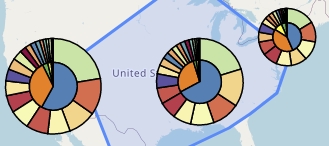
\includegraphics[width=0.5\textwidth]{highLevelUSA}
    \caption{Birds eye view USA}
    \label{fig:highLevelUSA}
\end{wrapfigure}

After starting the application for the first time you can see the glyphs. In the figure \ref{fig:highLevelUSA}, you can see the brirds eye view on the USA. It has there glyphs. Let's focus only on in the middle. The bluish area in the back with the blue border show the area which the glyph belongs to. This area shows up when you hover the mouse pointer over the respective glyph.
\\
From the outer circle of the glyph it you can see the relative appearance of the different UFO shapes. Meaning shape that is represented by the light green color is about one fourth of all UFO sighings.
\\
The inner circle does the same with the different types of airports.
\\

\begin{wrapfigure}{r}{0.6\textwidth} 
    \centering
    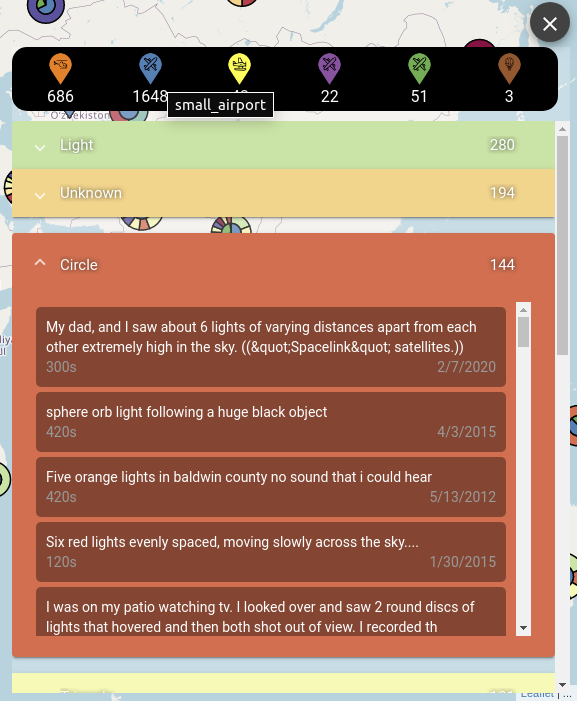
\includegraphics[width=0.5\textwidth]{legendEastCostUsa2}
    \caption{Legend of the East Coast USA glyph}
    \label{fig:legendEastCostUsa2}
\end{wrapfigure}

After clciking on the wished glyph a legend shows up. 
Now you can see more details about the glyph as shown in \ref{fig:legendEastCostUsa2}. 
The light green part of the outer circle represents 280 reporters claim that the shape 
of what they have seen was a light, 144 said it was a circle and 194 
didn't meantion a shape in their report. \\

Additionally you get more information about the airports which are within this area. In the 
black box on the top there are different airport markers. These represent the different kind of airports
that in this area. The number below the marker says how many there are of the specific type
in this area. For instance, the blue marker represents \textit{small airport}, the orange
one represents \textit{heliport} and so on. While hovering over the airport icon a tool tip
shows up that gives the textual representation of the airport type. Concrete this means there are 
1648 small airports, 686 heliports and various other different airports. 
\\
When clicking on a line inside the legend, meaning on a specific shape, a drop down opens and you
can see the different reports. Taking the first in figure \ref{fig:legendEastCostUsa2} inside circle
you have the report describtion 
\textit{My dad, and I saw about 6 lights of varying distances apart from each other extremely high in the sky…}
as well as the duration in the low left corner, \textit{300s} which means 300 seconds 
or 5 minutes, and the date it happend \textit{2/7/2020} in the right low corner. The date is in 
american format. Therefore it happend the February the 7th in 2020.
\\
\newpage
\begin{wrapfigure}{r}{0.6\textwidth} 
    \centering
    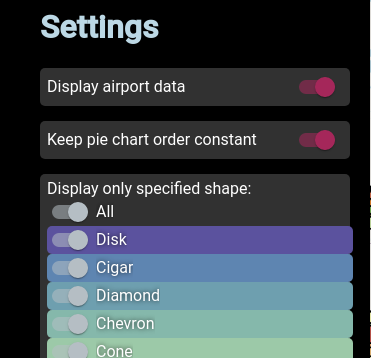
\includegraphics[width=0.5\textwidth]{SettingsTap}
    \caption{Legend of the East Coast USA glyph}
    \label{fig:SettingsTap}
\end{wrapfigure}

On the right left upper corner of the map there is a button with which you can open the settings.
Click on it the settings like shown in figure \ref{fig:SettingsTap} will slide in. Here you can fine tune
what you see on the map. \\
\textit{Display airport data}, with this slider you can show or hide the airport. From the high level view,
with the glyphs that doesn't alway make sence but when you have zoomed in it can happen that there
are more airports than sightings and maybe you want to see only the UFO sightings.
\\
The \textit{Keep pie chart order constant} is to fix the order of shapes of the glyph. The pie chart gives
shows the shape that occures the most first. If you want to compare two glyphs it can be useful to have the
shapes in a fixed order inside the glyphs.
\\
Finally there is the possiblity to include or exclude some shape. With this one you can
select the year range in which you want to explore sightings. 
\\


\begin{wrapfigure}{r}{0.6\textwidth} 
    \centering
    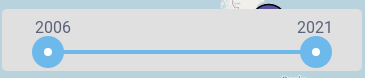
\includegraphics[width=0.5\textwidth]{yearSilder}
    \caption{Legend of the East Coast USA glyph}
    \label{fig:yearSilder}
\end{wrapfigure}

The last useful component is the year slider as shown in figure \ref{fig:yearSilder}. 
\\\\\\\\\\\\\\

\section*{Use Case}

Our world gets more an more filled with recommender systems, their only goal is to keep us looking at the screen. They show us things we might be interested in and they are very good at doing this. If one tends to believe in conspiracy theories the system will guide him towards new theories all the time.  \\
Our app could be one target such a person runs into. The diffenerce to any article they read is that form our app, this people will get a unfiltered non biased but accessible of browsing through these reports. They look at the single reports themselfs and decide if they think this is a trusty source or not. \\

\newpage

\begin{wrapfigure}{r}{0.7\textwidth} 
    \centering
    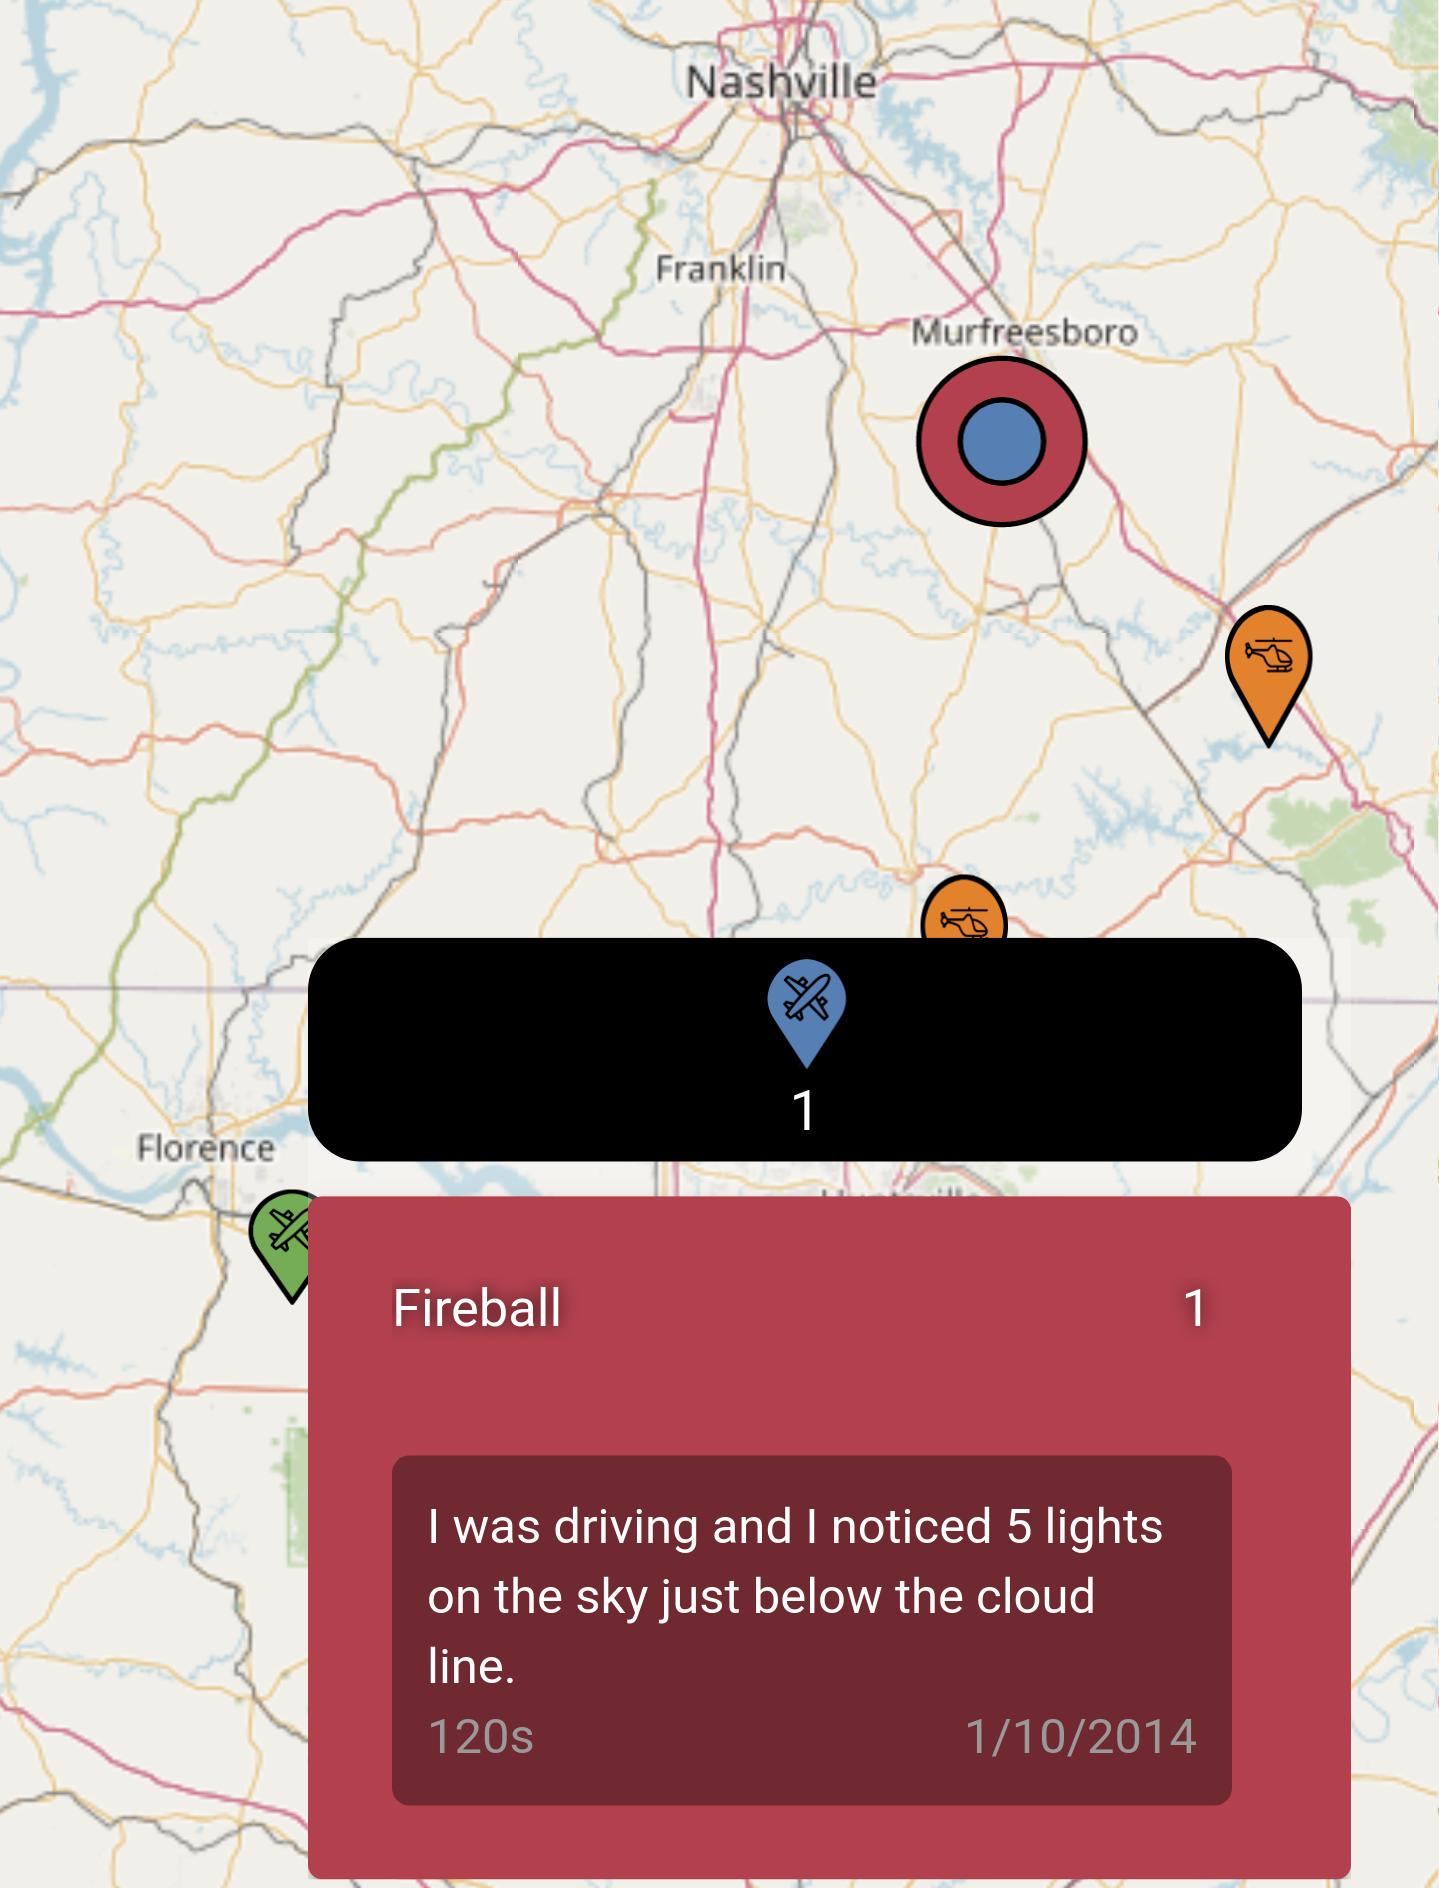
\includegraphics[width=0.4\textwidth]{Tennesee}
    \caption{Legend of the East Coast USA glyph}
    \label{fig:Tennesee}
\end{wrapfigure}

It could also be seen as a tool for scientific research or myth busting. Taking the 90s television series "X-Files", where two FBI agent investigate in unsolve cases that are weird due to their describtion. Actually it is not their goal to support some kind of mystic or supernatural theory.
They want to find proper and scientific bullet proof explanations for happenings. So do we! Always keep in mind it's easy to say that people haven't seen what they claim they did, but it's also possible that their interpretaion is simply wrong.

So let's say someone tells you he has see something weird in October 2014 near Nashville. You can double check with our app
if there is someone else that has seen the same phenomena. If yes might be worth spending some more time to Actually find out
what has happend that in this area.\\

\begin{wrapfigure}{r}{0.7\textwidth} 
    \centering
    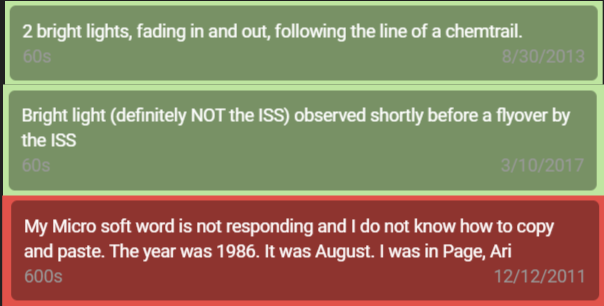
\includegraphics[width=0.4\textwidth]{funnyFindings}
    \caption{Legend of the East Coast USA glyph}
    \label{fig:funnyFindings}
\end{wrapfigure}

If you nither want to bust some myths nor you are open to conspiracy theories, 
you might use our app as we do. Click through the reports, look for the really 
stupid ones and read them loud to your friends. Like ones you can see in figure \ref{fig:funnyFindings}.
 Why? Because they are funny! Actually this is what this project is really about, "fun".

\end{document}
